\documentclass[../Main.tex]{subfiles}
\begin{document}
Interactions between particles are described by forces.
\section{Newton's Second Law}
\begin{definition}{Momentum}
    Momentum is equal to the product of mass and velocity:
    \begin{equation*}
        \vec{p} = m \dot{\vec{x}}
    \end{equation*}
    Where $m$ is the inertial mass.
\end{definition}
Mass is an additional property of point particles. It may be a function of time, though we will consider constant mass unless otherwise stated.\par
Then Newton's Second Law states that, in an inertial frame,
\begin{equation}
    \dot{\vec{p}} = \vec{F}.
    \label{eqnNewtonII}
\end{equation}
That is, the change in momentum is equal to the force.\par
The force $\vec{F}$ depends on the interactions but can only depend on $\vec{x}$ and $\dot{\vec{x}}$. This means that Newton's Second Law is a second-order differential equation for the vector $\vec{x}(t)$. So, given the position and velocity at some time for all particles in a system, $\vec{x}(t)$ is uniquely determined for all times.
\section{Conservative Forces and Gravity}
\subsection{Conservative Forces}
\begin{definition}{Conservative force}
    A force is \underline{conservative} if it can be written in the form:
    \begin{equation}
        \vec{F} = -\nabla V
        \label{eqnConservativeForce}
    \end{equation}
    For some potential $V(\vec{x})$, which is a scalar (with vector input).
\end{definition}
\subsection{Gravity}
For the rest of this subsection, we consider gravity as an example of a force.\par
The gravitational potential energy if a particle with mass $m$ at $\vec{x}$ due to another particle with mass $M$ at $\vec{x_0}$ is:
\begin{equation}
    V = \frac{-GMm}{|\vec{x} - \vec{x_0}|}
    \label{eqnGravitationalPotential}
\end{equation}
Then we need $\nabla V$, so we need $\nabla |\vec{x} - \vec{x_0}$:
\begin{align*}
    \partial_i (|\vec{x} - \vec{x_0}|^2) &= 2 |\vec{x} - \vec{x_0}| \partial_i |\vec{x} - \vec{x_0}| \\
    \partial_i (\vec{x} - \vec{x_0})_j (\vec{x} - \vec{x_0})_j &= 2 |\vec{x} - \vec{x_0}| \partial_i |\vec{x} - \vec{x_0}| \\
    2(\vec{x} - \vec{x_0})_j \partial_i (\vec{x} - \vec{x_0})_j &= 2 |\vec{x} - \vec{x_0}| \partial_i |\vec{x} - \vec{x_0}| \\
    (\vec{x} - \vec{x_0})_j \delta_{ij} &= |\vec{x} - \vec{x_0}| \partial_i |\vec{x} - \vec{x_0}| \\
    (\vec{x} - \vec{x_0})_i &= |\vec{x} - \vec{x_0}| \partial_i |\vec{x} - \vec{x_0}|
\end{align*}
Then rearranging for the required term:
\begin{equation}
    \nabla |\vec{x} - \vec{x_0}| = \frac{\vec{x} - \vec{x_0}}{|\vec{x} - \vec{x_0}|}
    \label{eqnDelSizeOfVec}
\end{equation}
Then using this result:
\begin{equation}
    \vec{F} = -\nabla V = -GMm \frac{\vec{x} - \vec{x_0}}{|\vec{x} - \vec{x_0}|^3}
    \label{eqnGravityTwoPoints}
\end{equation}
Or, if $\vec{r} = \vec{x} - \vec{x_0}$,
\begin{equation}
    \vec{F} = -\frac{GMm}{r^2} \uvec{r}
    \label{eqnGravitySeparation}
\end{equation}
We often write $V = m \Phi$, where $\Phi = -frac{GM}{|\vec{x} - \vec{x_0}}$ is the gravitational potential.
We can then consider an example:
\begin{example}[Motion on the surface of the earth]
    Near the surface of the earth, take $\vec{x_0}$ to be the centre of the earth, and $|\vec{x}| = R + z$, where $R$ is the radius of the earth, $R >> z$.
    \begin{align*}
        \Phi(R + z) &= -\frac{GM}{R + z} \\
        &= -\frac{GM}{R}(1 - \frac{z}{r} + \frac{z^2}{R^2} + O(z^3)) \\
        &\approx \text{ constant } + \frac{GMz}{R^2}
    \end{align*}
    So the force is $\vec{F} = -mg\uvec{z}$.\par
    This leads to the simplest possible motion due to a force:
    \begin{equation*}
        m\ddvec{x} = m \vec{g}
    \end{equation*}
    Then, taking the $z$ component:
    \begin{align*}
        \ddot{z} &= -g \\
        \dot{z} &= v_0 - gt \\
        z &= z_0 + v_0 t - \frac{1}{2}gt^2
    \end{align*}
\end{example}
\subsection{Energy}
Conservative forces have an associated energy that is conserved:
\begin{equation}
    E = \frac{1}{2} m \dvec{x} \cdot \dvec{x} + V(\vec{x})
    \label{eqnEnergy}
\end{equation}
Checking it is constant:
\begin{align*}
    \frac{dE}{dt} &= m \dot{x}_i \ddot{x}_j + \partial_i V \dot{x}_i \\
    &= \dot{x}_i \left(m\ddot{x}_i + \partial_i V\right) \\
    &= 0 \text{ by equation of gravity.}
\end{align*}
\begin{example}[Escape velocity]
    Escape velocity is the speed at which an object must be projected up such that it never falls back down.\par
    At the moment the object is thrown, the energy is:
    \begin{equation*}
        E_0 = \frac{1}{2} m v_0^2 - \frac{GMm}{R}
    \end{equation*}
    To not fall back, the object must reach $R \rightarrow \infty$ without velocity falling to 0.
    \begin{equation*}
        E_\infty = \frac{1}{2} m v_\infty^2 > 0
    \end{equation*}
    So we require $E_0 > 0$:
    \begin{align*}
        v_0^2 &> \frac{2GM}{R} \\
        v_0 &> \sqrt{\frac{2GM}{R}}
    \end{align*}
\end{example}
The mass $m$ cancelled because the gravitational mass, that appears in the force, is the same as the inertial mass that appears in the Second Law. The fact that these two are the same is called the Principle of Equivalence.\par
It is useful to write energy as $E = T + V$, where $T$ is the kinetic energy, and $V$ is the potential energy.\par
\begin{definition}{Work done}
    The \underline{work done}, $W$, is defined to be:
    \begin{equation}
        W = \int_{C} \vec{F} \cdot \vec{dx}
    \end{equation}
    It is a line integral.
\end{definition}
Conservative forces have the property that work done by the force as a particle moves along a trajectory depends only on the endpoints of the trajectory, not the specific path. There are two ways to see this.
\begin{align*}
    W &= \int_C \vec{F} \cdot \vec{dx} \\
    &= \int_{t_1}^{t_2} dt \vec{F} \cdot \dvec{x} \\
    &= m \int_{t_1}^{t_2} dt \ddvec{x} \cdot \dvec{x} \\
    &= \frac{m}{2} \int_{t_1}^{t_2} dt \frac{d}{dt}(\dvec{x}^2) \\
    &= T(t_2) - T(t_1) \\
    &= V(\vec{x}(t_1)) - V(\vec{x}(t_2)) \text{ by conservation of energy}
\end{align*}
Which only depends on the endpoints.\par
Note that the quantity $\vec{F} \cdot \dvec{x}$ is the power, $P$. It is the rate of change of doing work.\par
The second way is using a property of line integrals and gradients.
\begin{align*}
    W &= \int_C \vec{F} \cdot \vec{dx} \\
    &= -\int_C \nabla V dx \\
    &= V(\vec{x_1}) - V(\vec{x_2})
\end{align*}
\section{Motion in One Dimension}
Often, we can reduce problems to motion in one dimension. In one dimension, Newton's Second Law is:
\begin{equation}
    m\ddot{x} = F_x
    \label{eqnNewtonSecondOneDim}
\end{equation}
If $F_x$ is velocity independent, then it can always be written as a gradient of a potential:
\begin{equation}
    V(x) = -\int_{x_0}^{x} F_x(u) du
    \label{eqnPotentialOneDim}
\end{equation}
\subsection{Finding an Integral}
Then we can conserve an energy $E = \frac{1}{2} m \dot{x}^2 + V(x)$. Solving this as a first-order differential equation:
\begin{equation}
    t - t_0 = \pm \int_{x_0}^x \frac{du}{\sqrt{\frac{2}{m}\left(E - V(u)\right)}}
    \label{eqnTimeGivenEnergy}
\end{equation}
Such a formula is only easy to derive for 1 dimension. In more dimensions something like this may not even be possible to find. Even still, this integral is rarely solvable, especially for more complex systems.
\subsection{Potential and Stationary Points}
We can try to understand 1-dimensional motion without computing the integral in equation~\ref{eqnTimeGivenEnergy}. Considering the energy:
\begin{align*}
    E &= \frac{1}{2} m \dot{x}^2 + V(x) \\
    &\geq V(x) \text{ since the kinetic energy is} \geq 0
\end{align*}
So this restricts the places that a particle can be: for a particle of measured energy $E$, it cannot exist in such coordinates $x$ such that $V(x) > E$. Also, for coordinates $x$ such that $V(x) = E$, then $\dot{x}$ must equal 0 there. Such points are called turning points, because the particle must change direction at these points. \par
\begin{figure}[ht]
    \centering
        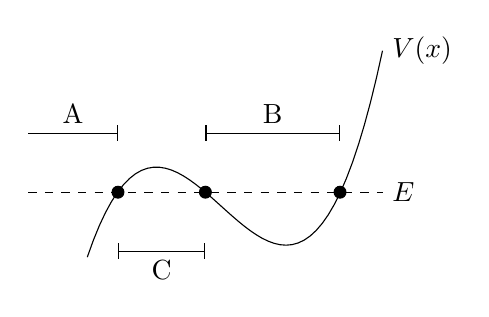
\begin{tikzpicture}[scale=1.5]
            \draw[domain=-0.5:2, samples=50] plot (\x, {\x * \x * \x -1.9 * \x * \x + 0.3 * \x + 1.2}) node[right] {$V(x)$};
            \draw[dashed] (-1, 1) -- (2, 1) node[right] {$E$};
            \draw[-Bar] (-1, 1.5) -- (-0.24, 1.5) node[pos=0.5, anchor=south] {A};
            \draw[Bar-Bar] (-0.24, 0.5) -- (0.5, 0.5) node[pos=0.5, anchor=north] {C};
            \draw[Bar-Bar] (0.5, 1.5) -- (1.64, 1.5) node[pos=0.5, anchor=south] {B};
            \foreach \x in {-0.24, 0.5, 1.64}
                \draw[fill] (\x, 1) circle[radius=0.5mm];
        \end{tikzpicture}
    \caption{Regions for a given potential and energy of a particle}
    \label{figPotentialPlot}
\end{figure}
In figure~\ref{figPotentialPlot}, we have two regions. In region B, the particle motion is of bouncing back and forth between the two turning points. In region A, the particle can reach the turning point, and then fly off to $-\infty$. The particle cannot exist in region C.\par
A special case occurs when $E = V(x)$ and furthermore $V'(x) = 0$. These are called equilibrium points. Here it is possible for the particle to lie stationary:
\begin{align*}
    V = E &\implies \dot{x} = 0 \\
    m\ddot{x} &= -V'(x) = 0
\end{align*}
And thus at an equilibrium point $\ddot{x} = \dot{x} = 0$.\par
Motion close to an equilibrium point is especially simple, depending only on the curvature of $V(x)$ around the stationary point. Let $x_0$ be the equilibrium point and $x$ be the position of a particle, where $x$ is close to $x_0$.
\begin{align}
    V(x) &= V(x_0) + (x - x_0)V'(x_0) + \frac{1}{2}(x - x_0)^2 V''(x_0) + O((x - x_0)^3) \nonumber \\
    &\approx V(x_0) + \frac{1}{2}(x - x_0)^2 V''(x_0) \label{eqnStationaryOneDimMotion}
\end{align}
In the case where $V''(x_0) > 0$, we have the potential for a harmonic oscillator:
\begin{equation*}
    m\ddot{x} = -V(x) \approx (x-x_0)V''(x)
\end{equation*}
And $x(t)$ gives small oscillations about $x_0$, with frequency $\omega = \sqrt{\frac{V''(x_0)}{m}}$.\par
In the case where $V''(x_0) < 0$, we have an unstable equilibrium point:
\begin{equation*}
    x = x_0 Ae^{\gamma t} + Be^{-\gamma t}
\end{equation*}
where $\gamma = \sqrt{-\frac{V''(x_0)}{m}}$. Solutions to $x(t)$, for $A \neq 0$, display exponential growth and are thus unstable. Solutions with $A = 0$ correspond to the ball having exactly enough energy to reach the equilibrium point and stop there.\par
In the case $V''(x_0) = 0$, higher-order terms are needed. If $V(x)$ is not twice-differentiable at $x_0$, special consideration is needed for the specific case.
\section{Electromagnetic Forces}
Forces that depend on velocity typically do not have a conserved energy. One important exception is the Lorentz force that an electromagnetic field exerts on a charged particle.
\begin{definition}{Lorentz force}
    The force experienced by a particle with charge $q$ and at position $\vec{x}$ is the Lorentz force:
    \begin{equation}
        \vec{F} = q\left(\vec{E}(\vec{x}) + \dvec{x} \times \vec{B}(\vec{x})\right)
        \label{eqnLorentzForce}
    \end{equation}
    Here $\vec{E}$ is the electric field, $\vec{B}$ is the magnetic field. We assume static fields (that do not depend on time).
\end{definition}
Also, the electric field is given by:
\begin{equation}
    \vec{E}(\vec{x}) = -\nabla \phi(\vec{x})
    \label{eqnElectricField}
\end{equation}
And $\phi$ is the electric potential.\par
In the electric field, the conserved energy is $E = \frac{1}{2} m\dvec{x}^2 + q\phi(\vec{x})$. Checking the field is conservative:
\begin{align*}
    \frac{dE}{dt} &= m\dvec{x} \cdot \ddvec{x} + q \nabla\phi \cdot \vec{x} \\
    &= \dvec{x} \cdot (\vec{F} - q\vec{E}(\vec{x})) \\
    &= \dvec{x} \cdot (q\vec{x} \times \vec{B}(\vec{x})) = 0
\end{align*}
The velocity-dependent force is orthogonal to the trajectory of the particle, and so does no work on the particle, and therefore energy is conserved.\par
The electric force is similar to gravitational force. The potential at $\vec{x}$ due to a particle of charge $Q$ at $\vec{x_0}$ is:
\begin{equation}
    \phi(\vec{x}) = \frac{Q}{4\pi \epsilon_0} \frac{1}{|\vec{x} - \vec{x_0}}
    \label{eqnElectricPotential}
\end{equation}
And therefore like gravity we have an inverse-square law, this is called the Coulomb Force.\par
One important difference between the gravitational force and the Coulomb force is that mass is always positive, so gravity is attractive. Charges can be positive or negative, and so the electric force can be attractive or repulsive.\par
Magnetic forces are different. A charged particle in a magnetic field obeys:
\begin{equation}
    m\ddvec{x} = q\dvec{x} \times \vec{B} \\
    \label{eqnMagneticForce}
\end{equation}
This is a vector differential equation. We solve for constant magnetic field. Align the coordinate system such that $\vec{B} = B\uvec{z}$. Also write $\vec{x} = (x, y, z)^T$.\par
Then solve equation~\ref{eqnMagneticForce} using this coordinate system:
\begin{align*}
    m\ddot{x} &= qB\dot{y} \\
    m\ddot{y} &= -qB\dot{x} \\
    m\ddot{z} &= 0
\end{align*}
Parameterising $m, q, B$ as $\omega = \frac{qB}{m}$ fully describes the system. $\omega$ is called the cyclotron frequency.\par
Solving the equation in $z$:
\begin{equation*}
    z = z_0 + v_z t
\end{equation*}
So we have constant-velocity motion in the $z$ direction.\par
Then we have a system of 2 equations to solve ($x$ and $y$). We can eliminate a variable:
\begin{align*}
    m \frac{d\ddot{x}}{dt} &= qb\ddot{y} \\
    &= -\omega^2 \dot{x} \text{ by substituting for } \ddot{y} \\
    \dot{x} &= \tilde{A}\sin{(\omega t + \phi)} \\
    x = x_0 + A \cos{(\omega t + \phi)}
\end{align*}
And we can solve for $y$:
\begin{equation*}
    y = y_0 - A \sin{(\omega t + \phi)}
\end{equation*}
And this motion is circular in the x-y plane, with constant velocity in the $z$ direction.\par
We can solve this in a much easier way using complex numbers.\par
Let $\xi = x + iy$. Now consider:
\begin{align*}
    \ddot{\xi} &= \ddot{x} + i\ddot{y} \\
    &= -i\omega \dot{\xi} \\
    \xi &= c_1 e^{-i\omega t} + c_2
\end{align*}
Then relabelling the constants as: $c_1 = Ae^{-\phi}, c_2 = x_0 + i y_0$, we get the solutions as above.
\section{Dimensional Analysis}
\label{sectDimAnalysis}
\begin{definition}{Dimensional analysis}
    \underline{Dimensional analysis} is the ability to remove constants from equations by rescaling variables.
\end{definition}
\begin{example}[Explicit dimensional analysis for a pendulum]
    Consider a pendulum: a light rod of length $l$ suspending a mass of length $m$ that makes an angle of length $\theta$ to the vertical. The gravitational field strength at this point is $g$.\par
    We know that the equation of motion is:
    \begin{equation}
        \frac{d^2\theta}{dt^2} = -\frac{g}{l}\sin{\theta}
        \label{eqnPendulumDiffEqn}
    \end{equation}
    We would like to know the period $T$ of the pendulum: $\theta(t + T) = \theta(T)$, where $T$ is the least such.\par
    We want to remove $g$ and $l$ from the equation. The only way to do this is by rescaling time (rescaling $\theta$ will not work):
    \begin{equation*}
        t = \sqrt{\frac{l}{g}}\tau
    \end{equation*}
    If we let $\theta(t) = \theta(t(\tau)) = F(\tau)$ equation~\ref{eqnPendulumDiffEqn} becomes:
    \begin{equation*}
        \frac{d^2 F}{dt^2} = -\sin{F}
    \end{equation*}
    Therefore the period $\Delta \tau$ of $F(\tau)$ may depend on initial conditions but cannot depend on $l$ and $g$.
    \begin{align*}
        &\implies F(\tau + \Delta\tau) = F(\tau) \\
        &\implies \theta(t) = F(\tau) = F\left(\sqrt{\frac{g}{l}}t\right) \\
        &= F\left(\sqrt{\frac{g}{l}}t + \Delta\tau\right) \\
        &= F\left(\sqrt{\frac{g}{l}}\left(t + \sqrt{\frac{l}{g}} \Delta \tau\right)\right) \\
        &= \theta\left(t + \sqrt{\frac{l}{g}}\Delta\tau\right) \\
        &\implies T = \sqrt{\frac{l}{g}} \Delta \tau \propto \sqrt{\frac{l}{g}}
    \end{align*}
    So without solving the equation, we know that the period of a pendulum is proportional to $\sqrt{l}$.\par
\end{example}
In general, the rescalings might not be obvious. We associate dimensions to constant and variables as a shorthand.\par
\begin{definition}{Dimension of a variable}
    We define any variable a \underline{dimension} based on the fundamental dimensions: length $L$, mass $M$, and time $T$.
\end{definition}
\begin{examples}{}
    \item $[\dot{x}] = LT^{-1}$,
    \item $[\ddot{x}] = LT^{-2}$,
    \item $[E] = ML^2 T^{-2}$
\end{examples}
For any physical equation, the dimension on the LHS and RHS must be equal. This implies that all arguments to non-linear functions must be dimensionless (for example $\sin$).
\begin{example}[Pendulum revisited]
    We have $[g] = LT^{-2}, [l] = L, [m] = M$. We want the period $T$ to have dimension time.\par
    Then $T = f(\theta) g^A l^B m^C$ for constants to be determined. This gives:
    \begin{align*}
        [T] &= [g]^A[l]^B[m]^C \\
        T &= L^A T^{-2A} L^B M^C
    \end{align*}
    which gives $A = -\frac{1}{2}$, $B = \frac{1}{2}$, $C = 0$.
\end{example}
\section{Friction}
When objects move through a medium, there are many microscopic forces between the object and the particles of its medium. These cause momentum to be carried off into the medium. This momentum is called heat, and is lost.
\subsection{Types of Friction}
\begin{definition}{Friction}
    \underline{Friction} is the macroscopic force that keeps track of the momentum lost due to complicated microscopic effects.
\end{definition}
We require it to have some properties:
\begin{itemize}
    \item Does not conserve the energy of the object (energy lost as heat)
    \item Friction is irreversible (no energy gain from friction). It is antiparallel to $\dvec{x}$.
\end{itemize}
Thus the two simplest cases that describe friction are:
\begin{definition}{Linear drag}
    A representation of friction that is linear in the velocity is \underline{linear drag}:
    \begin{equation}
        \vec{F} = -k\dvec{x}
        \label{eqnLinearDrag}
    \end{equation}
\end{definition}
\begin{definition}{Quadratic Drag}
    We can also have a friction proportional to the square of the velocity, \underline{quadratic drag}:
    \begin{equation}
        \vec{F} = -k|\dvec{x}|\dvec{x}
        \label{eqnQuadraticDrag}
    \end{equation}
\end{definition}
Quadratic drag can arise as we have one factor of $\dvec{v}$ in the rate of collision with medium particles, and the other factor in the amount of momentum lost per collision. Also, the number of collisions should be proportional to the density of the medium, $\rho$, and the frontal area $A$ of the object. Therefore $k \propto \rho A$.\par
Dimensional analysis: $[F] = MLT^{-2}$, and $[kv^2] = ML^{-3}L^2L^2T^{-2} = MLT^{-2}$. So any other factor in this constant is dimensionless.\par
Linear drag is slightly harder: it comes from viscous effects (the \textit{stickiness} of a medium). The linearity in $\dvec{x}$ comes from the particle dragging the particles of the medium with it. The required result is Stokes' Law: for a spherical object of radius $l$ in fluid of viscosity $\eta$, the required constant $k$ is $6\pi L\eta$.\par
Whether quadratic or linear drag is more important is dependent on the Reynold's Number:
\begin{equation*}
    R = \frac{\rho v L}{\eta} = \frac{F_{\text{quadratic}}}{F_{\text{linear}}}
\end{equation*}
Which describes the relative importance of quadratic and linear drag.\par
We also have another type of friction:
\begin{definition}{Dry Friction}
    When one object is in contact with another, we can represent this object with dry friction. See chapter~\ref{chapRigidBodies}.
\end{definition}
\begin{example}[Terminal velocity]
    Consider a particle falling under gravity and under the influence of quadratic friction.\par
    Consider only motion in one dimension (radial with respect to the gravitational field).
    \begin{equation*}
        m\ddot{x} = -mg + k \dot{x}^2
    \end{equation*}
    We can consider this a differential equation in $v = \dot{x}$:
    \begin{equation*}
        m\frac{dv}{dt} = kv^2 - mg
    \end{equation*}
    Then we have a stable fixed point when $v = -\sqrt{\frac{mg}{k}}$. This is known as the \underline{terminal velocity}. For a raindrop, this is about $10 m s^{-1}$.\par
    The time taken to reach terminal velocity can be considered by dimensional analysis:\par
    Let $T = f(m, g, k)$, so $T \propto M^A L^B T^{-2B} M^C L^{-C}$. Solving this gives:
    \begin{equation*}
        T \propto \sqrt{\frac{m}{kg}}.
    \end{equation*}
    For a raindrop, this is around 1 second.
\end{example}
\subsection{Damping}
Friction damps small oscillations about an equilibrium point.\par
For small oscillations, linear drag is more important and the equation of motion is:
\begin{equation}
    \ddot{x} = -\omega_0^2 x - 2\alpha\dot{x}
    \label{eqnDamptedOscillation.}
\end{equation}
In IA Differential Equations, we considered 3 types of motion:
\begin{enumerate}
    \item \underline{Underdamping}: oscillations that decay slowly
    \item \underline{Critical damping}: The shortest time for the particle to return to equilibrium
    \item \underline{Overdamping}: A slow exponential decay to the equilibrium
\end{enumerate}
\end{document}